\section{Experimental Design}

\subsection{Metric performance}
This experiment aims to reduce the number of metrics to assess in the later rounds. The thinning out of metrics is required due to limited resources. Therefore, possible further work could involve repeating this work with a much more varied selection of metrics. The chosen metrics up for assessment are Soundex, Metaphone, NYSIIS, Levenshtein and Phonetic vectors.
\\\\
The design for the experiment involves assessing the quality of the metrics matches by having participants rate them on a scale of 1 (Very different sound) to 5 (Very similar sound).

\subsubsection*{Comparisons}
Each comparison contains a match-pair. These matches are generated by running the similarity metric over all the pairings in the Trustword dictionary. If two words are deemed a match they are added to their own list. Potential matches are then sampled from their respective lists.

Each participant is then asked to rate the similarity of a match on a scale of 1 (\textit{`Very different sound'}) and 5 (\textit{`Very similar sound'}). Figure \ref{fig:phoneticMatch} shows an example match and the connected scale. Users are provided with five of these comparisons per similarity metric.

\begin{figure}[h!]
    \centering
    \begin{adjustbox}{width=0.5\textwidth,center}
        \fbox{
        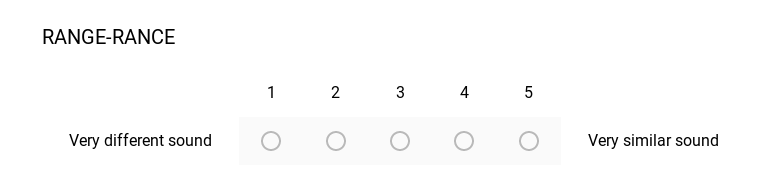
\includegraphics[width=\textwidth]{experiment/experiment_match.png}
        }
    \end{adjustbox}
    \caption{Example experiment question}
    \label{fig:phoneticMatch}
\end{figure}

The experiment randomises the order of these comparisons per session alongside a complete refreshing of matches once per submission. This design makes sure selections from the samples are fair and consistent as each user has a different selection of matches.

\subsubsection*{Quality control}
\label{sec:exp1_qualitycontrol}
As the study was being outsourced to Amazon's Mechanical Turk, the requirement to check the quality of results is essential. Therefore, a couple of additions were provided to check a result's validity.

The first was the addition of five "Random matches" questions. These are matches consisting of two random words selected from the dictionary. Therefore, the expected average rating of these words should be close to one. This design allows for a simple check for valid results. If their average rating for Random matches is too high, their results are discarded.

Alongside this, was the addition of two questions comparing precisely the same word. As both words are the same, the result should always be a full 5/5 rating, any results without a full rating are discarded. Figure \ref{fig:exactMatch} contains one example of the attention question used to filter inaccurate results.

\begin{figure}[h!]
    \centering
    \begin{adjustbox}{width=0.5\textwidth,center}
        \fbox{
            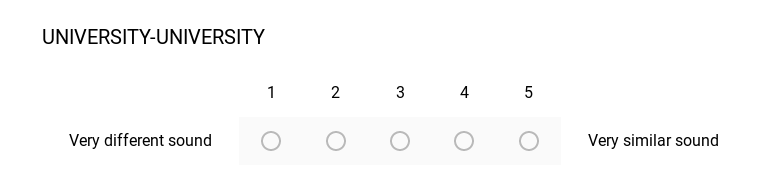
\includegraphics[width=\textwidth]{experiment/exact_experiment_match.png}
        }
    \end{adjustbox}
    \caption{Exact experiment attention question}
    \label{fig:exactMatch}
\end{figure}

The final check to ensure the validity of results is a check for native English fluency. Having non-native English speakers complete the 
experiment can introduce inconsistencies into the 
data and, therefore, needs to remain controlled. To achieve this, a preliminary MTurk study has been created to ask users for their perceived 
English fluency on a scale of 1 (Basic Understanding) to 5 (Native). 
Workers with an answer of 5 are provided with a 
Qualification
that tags them as defining themselves as native speakers. This qualification is then 
added as a prerequisite when running the experiment. This prerequisite ensures 
only fully native speakers are being assessed. The possibility of the 
worker falsely stating their level of fluency has also been considered. 
However, as the worker does not know the purpose of this initial study,
thereby providing inaccurate results has no real valid motive for the 
worker.

% TODO: Consideration section?

\subsection{Trustword Attacks}
\label{sec:exp2_design}

This experiment is designed to be a simulation of the attack proposed in Section \ref{sec:attackDesign}. The experiment tests the simulated matches of three similarity metrics decided by the previous experiment. The overall aim of the experiment is to quantify the success rate of the attack on live participants. Figure \ref{fig:trustwordUI} contains a view of the user interface used in the experiment. It has been designed to be as similar as the \pep Android application.

\begin{figure}[h!]
    \centering
    \begin{adjustbox}{width=0.4\textwidth,center}
        \fbox{
            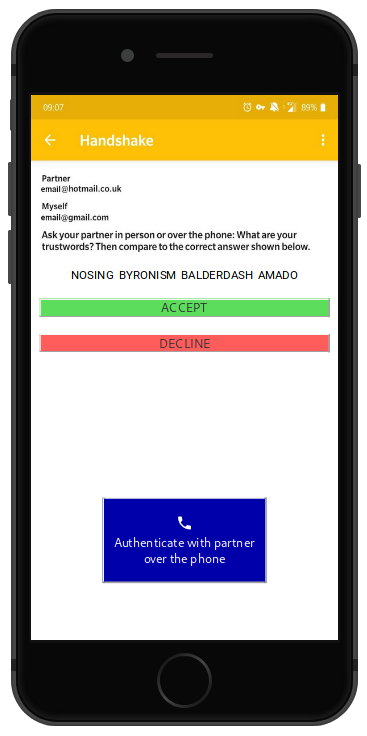
\includegraphics[width=\textwidth]{experiment/trustword_attack.png}
        }
    \end{adjustbox}
    \caption{Trustword user interface}
    \label{fig:trustwordUI}
\end{figure}


A live version of the application is avaliable\footnote{\url{https://afray.pythonanywhere.com/}}. The blue button is clicked to simulate the authentication ceremony over the phone. A text-to-speech system then reads a set of words. The user should accept if they match and decline if they don't.

\subsubsection{Design}

Due to the scarcity of attacks in a real-world setting, users are often complacent about their occurrence. Therefore, in this experiment, attacks only occur 30\% of the time. This occurrence is a much higher value than in a real-world setting but is a balance between resources and realistic design. If the chosen attack rate is too low, many more trials are required to collate a useful number of attack instances, thus, requiring more resources, but with more realism. If, however, the attack rate is too high, less total rounds are required to obtain the target number of attack trails. However, the user's complacency is lost as an attack is expected. This loss of complacency is undesirable as it does not realistically reflect real life. Furthermore, the first 5 trials of a new experiment are always benign. This inclusion is to ensure users are consistently lulled into complacency.

Certain keys have higher levels of potential near-collision keys than others due to how certain words are deemed similar by the similarity metric. Therefore, if random sets of words are chosen with no restraints, there are attacks presented to the user that in a real setting would be infeasible as they are close to a $2^{64}$ attack (4 Words * 16-bits). Therefore, the experiment is designed to sample from a list of "vulnerable" keys. These are keys that have a number of potential near-collision keys that allow computation in a specified timeframe. 

Furthermore, certain levels of attacks are also simulated. Below is the list of attacks considered in this experiment: 

\begin{itemize}
    \item (\OOOO) All words in the set can vary             
    \item (\XOOO) All but the first word can vary           
    \item (\XOOX) All but the first and last word can vary  
\end{itemize}

$Where: $
\begin{itemize}
    \item[] \verb|X|: is a static word
    \item[] \verb|O|: is a changeable word
\end{itemize}

The start and ends were chosen as the highest priority words to keep static. This design choice is due to research highlighting the common habit of users only to check the start and end of a checksum. 

These attacks are ascending in complexity. The timeframe for computing a near-collision was decided as one week with attack strengths of 7 GPU-days \textit{(1 x GPU)}, 70 GPU-days \textit{(10 x GPUs)} and 700 GPU-days \textit{(100 x GPUs)} on a mid-range GPU (AMD RX 480). Due to the long lifetime of PGP keys, 7 days was chosen as a reasonable length of the attack. The tool requires no user interaction once started, therefore, it can be left for an extended period to compute potential keys. This timeframe is also a maximum time, as these attacks also include keys that have a shorter average computation time.

% \begin{table}[h!]
%     \centering
%     \begin{tabular}{lll}
    GPU/days & No of combinations required & Attack Type \\
    \hline
    1       & 15250   & Zero static\\
    10      & 1525    & One static\\
    100     & 152     & Two static\\        
\end{tabular}
%     \caption{Summary of attack requirements}
%     \label{tab:attackReq}
% \end{table}

Table \ref{tab:attackReq} contains a summary of the different level of attacks and their respective restrictions. Any key that exceeds the defined numbers of potential near-collision key for attack level is deemed as vulnerable. A list of these vulnerable keys is sampled from when an attack is simulated.

\subsubsection{Quality control}
\label{sec:exp2_quality}
Like the previous experiment, participants are sourced from MTurk. Therefore, again, quality control is an aspect that requires consideration. As with the previous study, initially screened native speakers are used. Alongside this, two metrics are used to detect invalid results: audio-button-clicks and the overall-time. 

Audio-buttons-clicks is the number of times the blue \textit{"Authenticate with partner over the phone"} button in Figure \ref{fig:trustwordUI} is clicked. If there are rounds without button clicks, this is a sign of non-attentiveness. The design choice was made to allow non-clicks. This design provides a way to detect and discard click-throughs\footnote{Workers that aim to complete the task as fast as possible, with no regard for the quality of responses}. 

Overall-time is as the name suggest a recording of the time taken to complete the entire experiment. If users complete the experiment in an abnormally small amount of time, it can be used as another detection for invalid responses. A benchmark for the time is set by completing the experiment as fast as possible. Anything quicker was discarded as anything faster risks invalid and rushed results.